\documentclass{article}
\usepackage{graphicx}
\usepackage[section]{placeins}
\title{ Water Surface Garbage Collector System 
\linebreak
\\
\large EYIC Team ID 678
}
\date{2019-12-5}
\author{Gaurav, Nadeem, Ujjawal}

\begin{document}

\maketitle
\pagenumbering{gobble}
\pagenumbering{arabic}

\newpage
\section{Introduction}
In this fastest growing world, we are forgetting the nature and degrading it in several ways. 
For specific plastic is non bio degradable object that is thrown in the aquatic ecosystem, that is leading to degradation of marine habitat and also affecting human life. The main focus is to enhance the life of aquatic species.
\linebreak
\linebreak

\section{Market Research}
\begin{itemize}
	\item 40 percent of world’s water is polluted and unsafe for drinking
	\item 30 percent of people is dependent on water bodies for their occupations.
	\item Each year around 14 billion pounds of plastics are dumped into the water bodies.
	\item Untreated waste is dumped into water around 1.2 trillion gallons every year.
	\item 47 percent people will suffer to find drinking water by 2050.
\linebreak
\linebreak
\end{itemize}


\section{Hardware Requirements}
\begin{itemize}
	
	\item pipe * 4
	\item Bearings *4
	\item Net
	\item Lithium Ion Battery (11.6V, 4 Amp)
	\item Power Bank (5V)
	\item USB Camera
	\item Raspberry Pi
	\item Nodemcu Esp8266
	\item Motor 60 RPM * 2
	\item Motor 100 RPM * 2
	\item Motor Driver * 2
	\item Sun Board
	\item Servo Motor(SG-90) * 2
	\item Servo Motor(MG-995)
\newline
\newline
\end{itemize}

\section{Software Requirements}
\begin{itemize}
	\item Arduino IDE
\newline
\newline
\end{itemize}


\section{Implementation}
In this system, there are three phases –
\newline
\begin{enumerate}
	\item Detection of Waste – For the detection of waste, the camera is installed in the system so that user can easily monitor the location of waste. The output screen is built in the remote controller that is used to control the system in every possible direction.
	\item Extraction of Waste – The detected waste is then carried to the system by using conveyor belt fixed with the net that will segregate the waste and water.
	\item Collection of waste – The extracted waste is then travelled to the external net that is added at the back of the system, so that there is no effect of the weight on the system.
\end{enumerate}

\newpage
\section{Diagram}
\begin{figure}[!htb]
	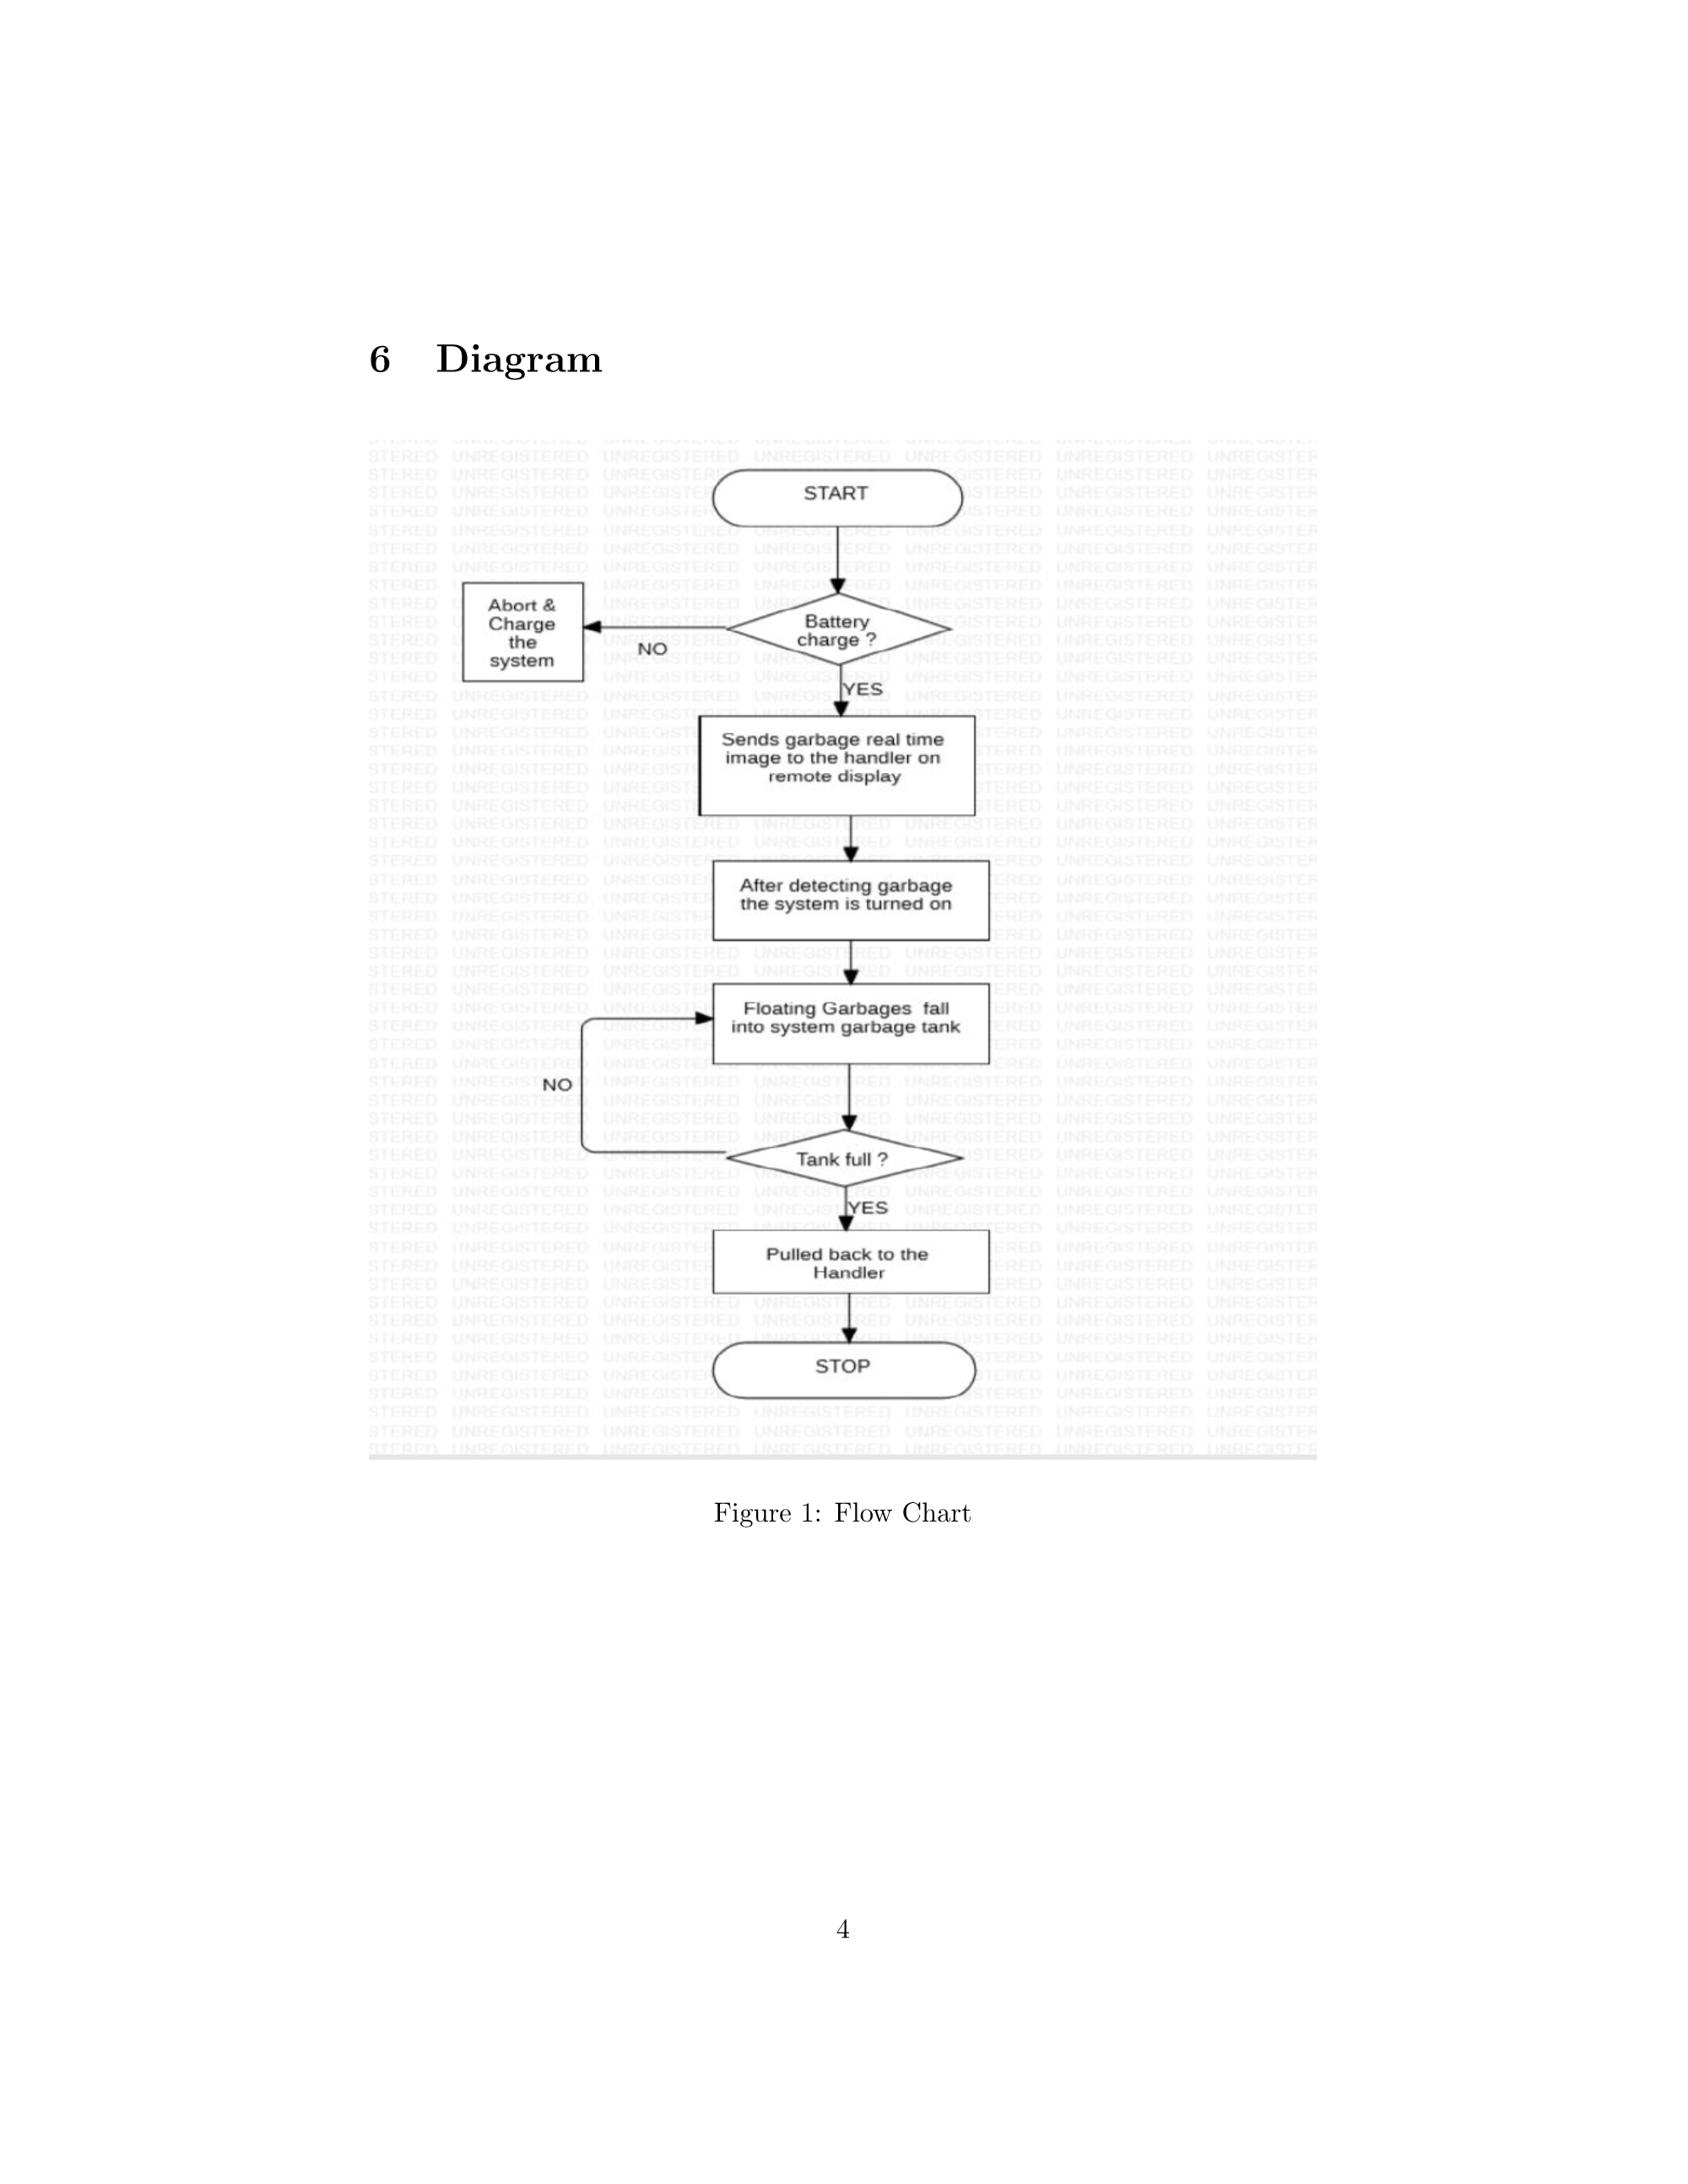
\includegraphics[width=\linewidth]{flowchart.png}
	\caption{Flow Chart}
\end{figure}
\begin{figure}
	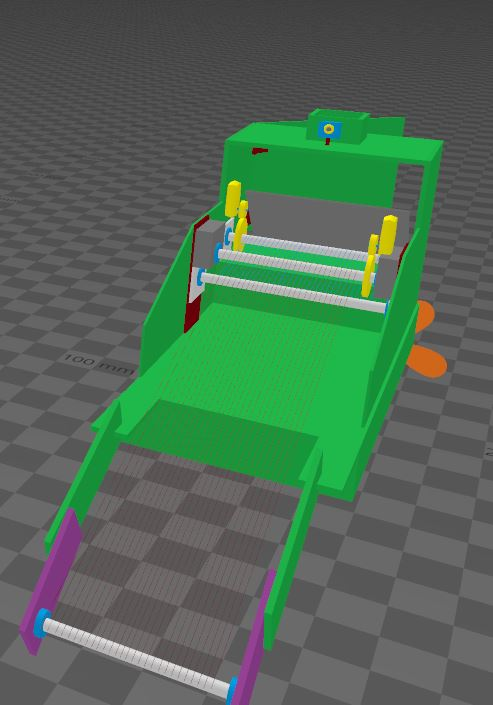
\includegraphics[width=\linewidth]{model.jpg}
	\caption{Model}
\end{figure}

\section{Feasiblity Study}
In the current scenario the plastic pollution is major concern in marine environment, as it is degrading their habitats. The 80 percent of the world’s wastewater is flow back into the water bodies without being treated and the huge amount of plastic waste is dumped by the humans directly into the water bodies. Since Earth contains 70 percent of water, it is not possible to clean the water manually, also it affects the health of the human being that is cleaning the water. An automation system is required to collect all the plastic wastes from the surface, which will enhance the life of the aquatic species as well as the people that are depends on the ````````````````````````````````````````````````````````````````````````````````````````occupations and the people living nearby that area. This automation system will decrease the manpower and give the possible results.
\end{document}